\documentclass{beamer}

\usepackage[utf8]{inputenc}
\usepackage{hyperref}

\usetheme{Berkeley}
\beamertemplatenavigationsymbolsempty
\setbeamertemplate{headline}{}
 
\title{FoodChain-Lab Installation}
\date{}
 
\begin{document}
\maketitle
 
\section{1}
\begin{frame}
	\begin{center}
  		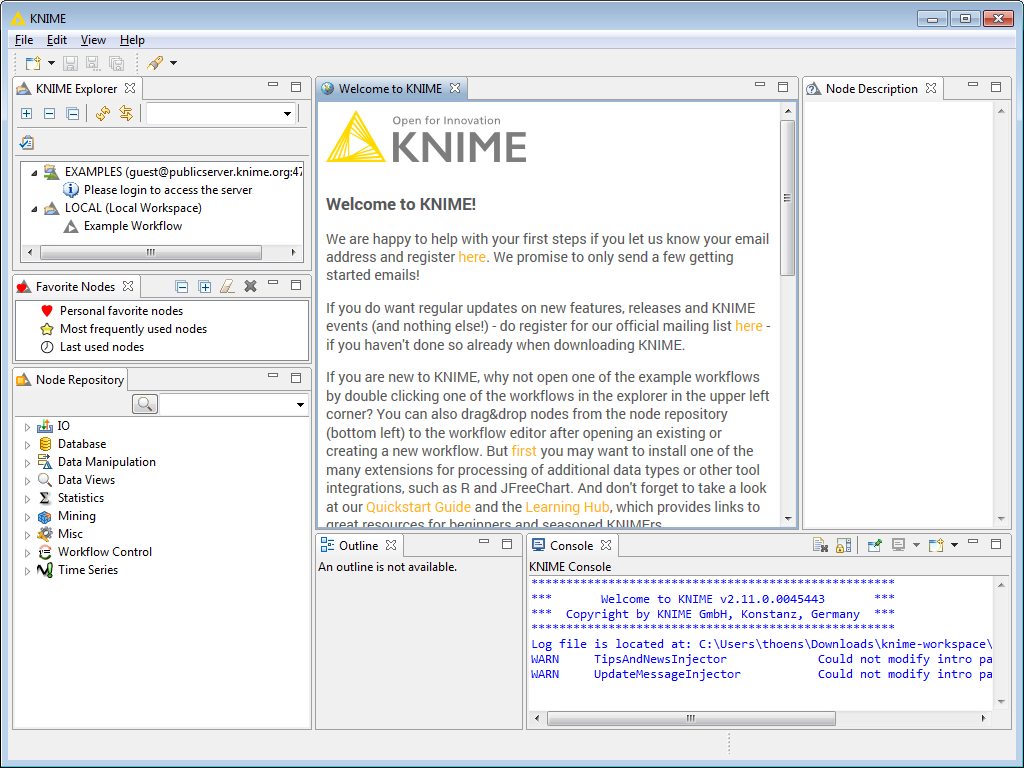
\includegraphics[height=0.6\textheight]{1.png}
	\end{center}
	\begin{itemize}
		\item Um FoodChain-Lab benutzen zu können, installieren Sie bitte zuerst die kostenlose Datenanalyse-Software KNIME (\url{https://tech.knime.org/installation-0}).
		\item Beim ersten Start von KNIME sieht die Benutzeroberfläche folgendermaßen aus.
	\end{itemize}
\end{frame}

\section{2}
\begin{frame}
	\begin{center}
  		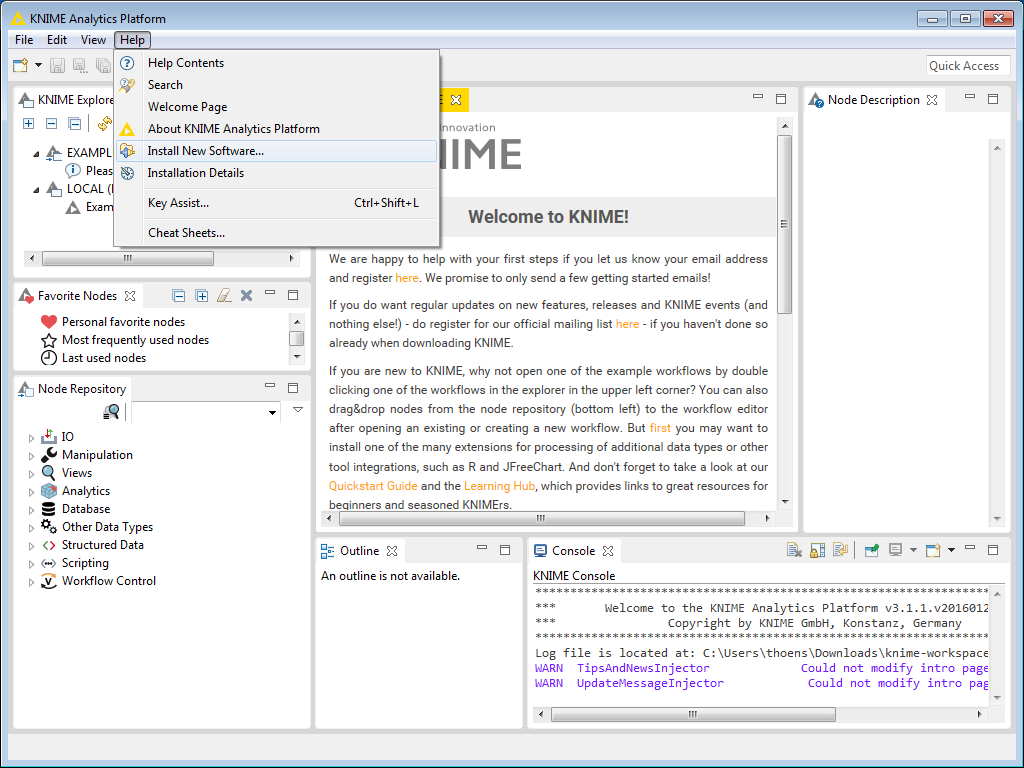
\includegraphics[height=0.7\textheight]{2.png}
	\end{center}
	\begin{itemize}
		\item Klicken Sie im Menü auf \textbf{Help $>$ Install New Software}.
	\end{itemize}
\end{frame}

\section{3}
\begin{frame}
	\begin{center}
  		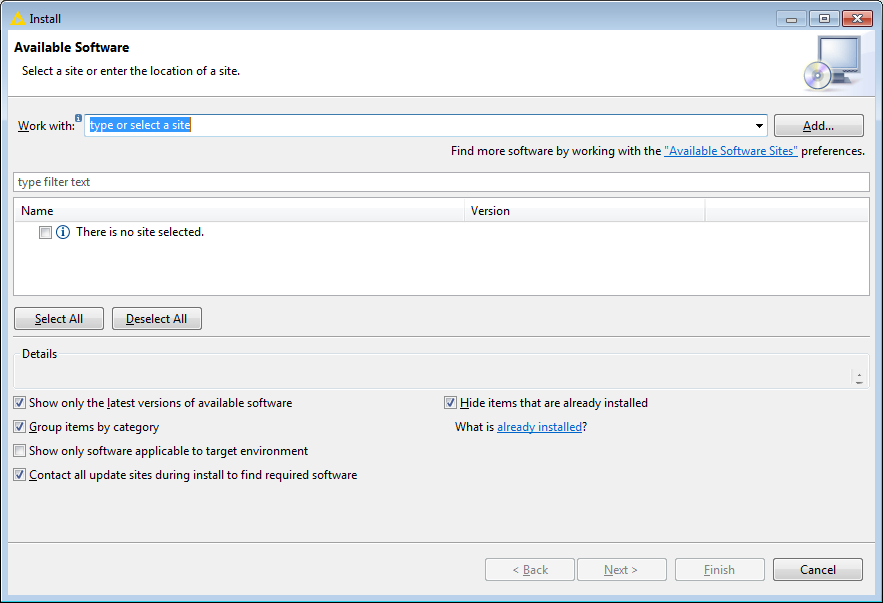
\includegraphics[height=0.7\textheight]{3.png}
	\end{center}
	\begin{itemize}
		\item Klicken Sie oben rechts auf \textbf{Add}.
	\end{itemize}
\end{frame}

\section{4}
\begin{frame}
	\begin{center}
  		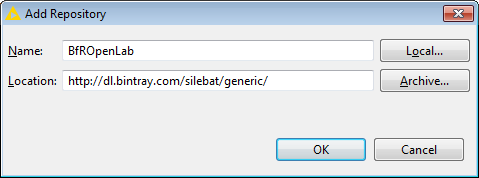
\includegraphics[width=0.9\textwidth]{4.png}
	\end{center}
	\begin{itemize}
		\item Im dann erscheinenden Add Repository Dialog geben Sie bitte "BfROpenLab" als Name und folgendes bei Location ein: \url{http://dl.bintray.com/silebat/generic/}
		\item Bestätigen Sie mit \textbf{OK}.
	\end{itemize}
\end{frame}

\section{5}
\begin{frame}
	\begin{center}
  		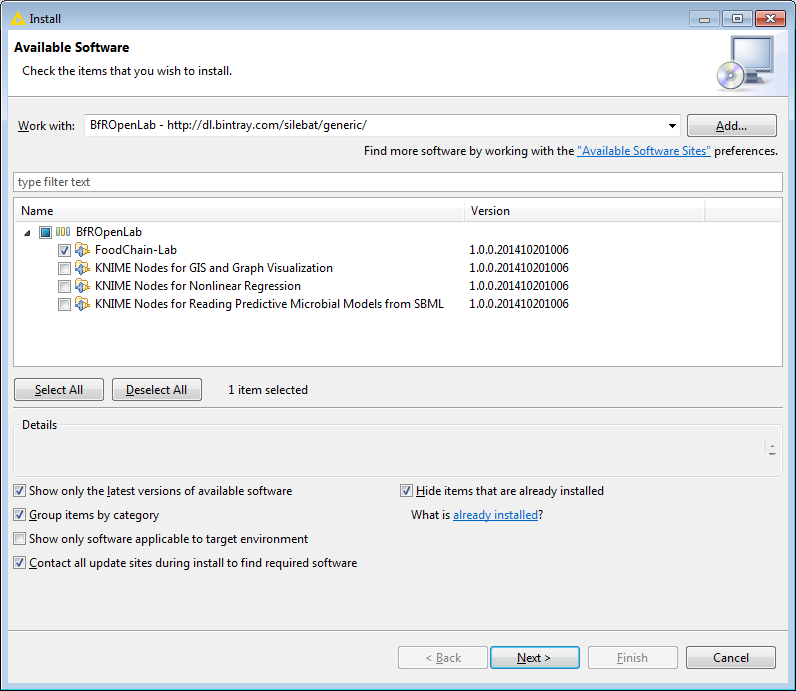
\includegraphics[height=0.7\textheight]{5.png}
	\end{center}
	\begin{itemize}
		\item Im Dialog "Available Software" klicken Sie bitte auf den Pfeil neben dem Kästchen bei "BfROpenLab" und wählen Sie "FoodChain-Lab" aus.
		\item Klicken Sie auf \textbf{Next}.
	\end{itemize}
\end{frame}

\section{6}
\begin{frame}
	\begin{center}
  		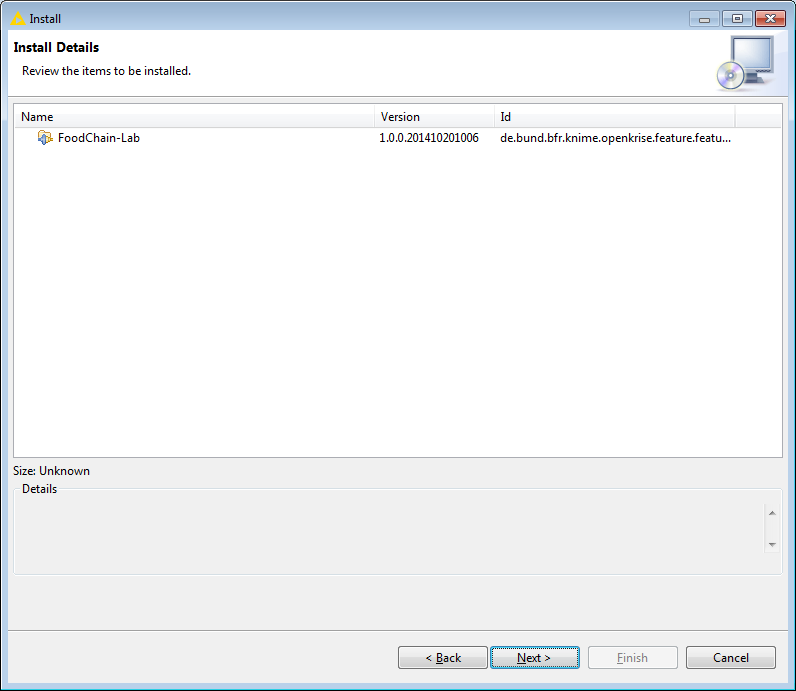
\includegraphics[height=0.7\textheight]{6.png}
	\end{center}
	\begin{itemize}
		\item Im folgenden Installationsmenü wird noch einmal aufgeführt, was nun installiert werden kann. Klicken Sie auf \textbf{Next}.
	\end{itemize}
\end{frame}

\section{7}
\begin{frame}
	\begin{center}
  		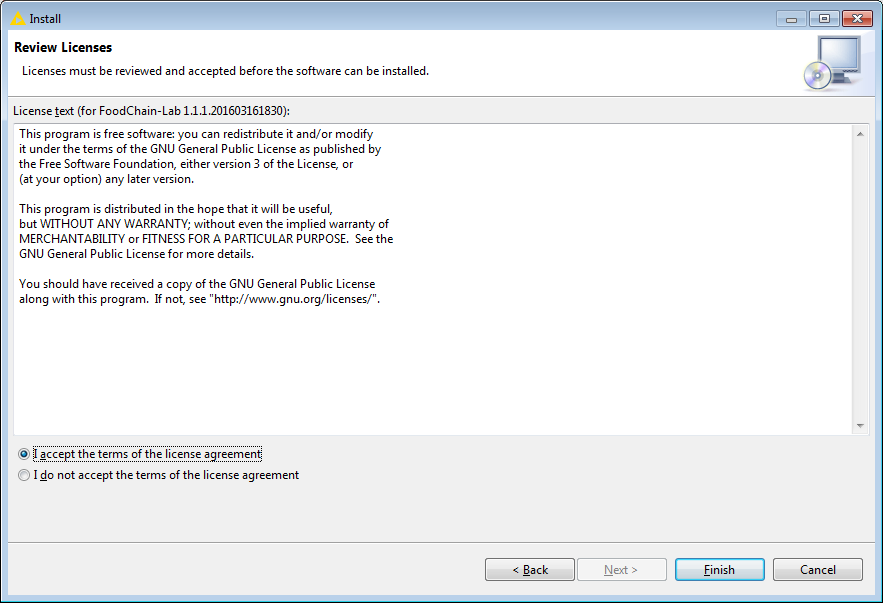
\includegraphics[width=0.7\textwidth]{7.png}
	\end{center}
	\begin{itemize}
		\item Lesen und akzeptieren Sie die Lizenzvereinbarung und klicken Sie anschließend auf \textbf{Finish}.
	\end{itemize}
\end{frame}

\section{8}
\begin{frame}
	\begin{center}
  		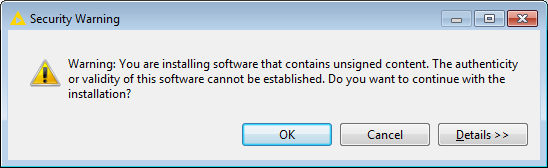
\includegraphics[width=0.9\textwidth]{8.png}
	\end{center}
	\begin{itemize}
		\item Sollten Sie eine Sicherheitswarnung erhalten, weil die Authentizität oder Validität der Software nicht ermittelt werden kann, klicken Sie bitte auf \textbf{OK}.
	\end{itemize}
\end{frame}

\section{9}
\begin{frame}
	\begin{center}
  		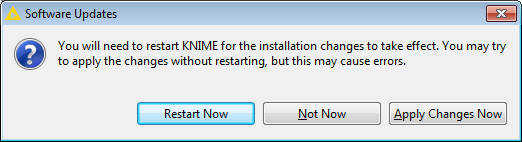
\includegraphics[width=0.9\textwidth]{9.png}
	\end{center}
	\begin{itemize}
		\item Nach der Installation starten Sie bitte KNIME neu (klicken Sie auf \textbf{Restart}).
	\end{itemize}
\end{frame}

\section{10}
\begin{frame}
	\begin{center}
  		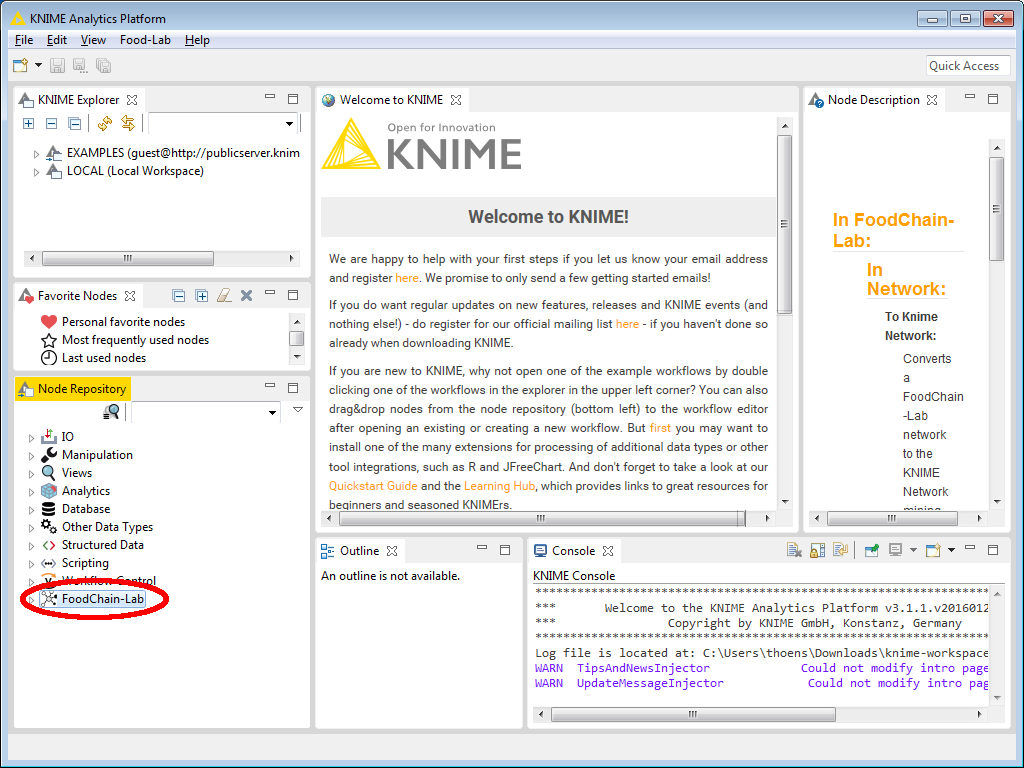
\includegraphics[height=0.6\textheight]{10.png}
	\end{center}
	\begin{itemize}
		\item Nach dem Öffnen von KNIME finden Sie die FoodChain-Lab-Knoten im \textbf{Node Repository} unten links.
	\end{itemize}
\end{frame}

\end{document}